\section{Half-wave and quarter-wave identities}

Two classical design identities of single-layer interferometry are checked
at the design wavelength $\lambda_0 = \SI{550}{\nano\metre}$. Both use a
three-layer stack (incident medium, film, substrate) at normal incidence
and are scanned across \SIrange{400}{800}{\nano\metre} for context.

The first panel realises the half-wave \emph{invisible} layer: a lossless
film of index $n_f = 2.0$ is placed on glass ($n_s = 1.5$) in air
($n_0 = 1.0$), with thickness
\begin{equation}
  d_{\rm HW} = \frac{\lambda_0}{2 n_f} = \SI{137.5}{\nano\metre}. \label{eq:hw-d}
\end{equation}
At $\lambda_0$ the film introduces a round-trip phase of $2\pi$, so the
internal Airy factor in~\eqref{eq:airy-r} reduces to unity and the
reflectance of the stack at that wavelength collapses to the bare-substrate
value,
\begin{equation}
  R(\lambda_0) = \left(\frac{n_0 - n_s}{n_0 + n_s}\right)^{2}. \label{eq:hw-R}
\end{equation}

The second panel realises the index-matched quarter-wave antireflection
(AR) film: the film index is chosen as the geometric mean
$n_f = \sqrt{n_0 n_s} \approx 1.225$, the thickness is
\begin{equation}
  d_{\rm QW} = \frac{\lambda_0}{4 n_f}, \label{eq:qw-d}
\end{equation}
and~\eqref{eq:airy-r} then gives exact destructive interference at
$\lambda_0$,
\begin{equation}
  R(\lambda_0) = 0. \label{eq:qw-R}
\end{equation}

\begin{center}
\begin{tikzpicture}
  \fill[black!4] (0, 0) rectangle (5, 1.6);
  \fill[green!10] (0,-0.7) rectangle (5, 0);
  \fill[blue!6]  (0,-1.9) rectangle (5,-0.7);
  \draw[thick] (0,0) -- (5,0);
  \draw[thick] (0,-0.7) -- (5,-0.7);
  \node[lbl, anchor=east] at (4.9, 1.2) {$n_0$};
  \node[lbl, anchor=east] at (4.9,-0.35) {$n_f$, $d$};
  \node[lbl, anchor=east] at (4.9,-1.4) {$n_s$};
  \raysketch{1.6}{0}{f}
\end{tikzpicture}
\end{center}

\begin{figure}[!htbp]
  \centering
  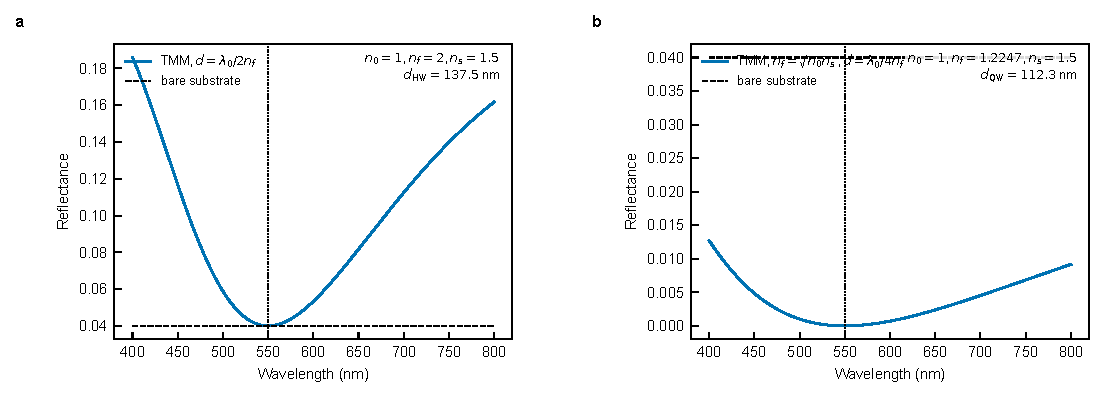
\includegraphics[width=\textwidth]{05_halfwave_quarterwave.pdf}
  \caption{(a) Half-wave invisible film returns the bare-substrate reflectance at $\lambda_0$. (b) Index-matched quarter-wave antireflection film gives zero reflectance at $\lambda_0$ and a smooth V-shape across the scan.}
  \label{fig:hwqw}
\end{figure}

At $\lambda_0$ the half-wave film coincides with the bare substrate to
$|R_{\rm film}(\lambda_0) - R_{\rm bare}| \approx \num{3e-17}$, and the
index-matched quarter-wave film reaches $R(\lambda_0) \approx \num{6e-33}$;
the latter is a squared amplitude and therefore registers the reflection
amplitude itself vanishing at the level of $\sqrt{\num{6e-33}} \sim
\num{8e-17}$, i.e.\ pure floating-point zero. The two identities
constrain the Airy phase and the Fresnel zero condition independently, so
their simultaneous satisfaction is a stronger check than either one alone.


